\chapter{Related Work}

There are a lot of algorithms which focus on image similarity and key feature detection, my main goal being to select specific ones on which we can control the sensitivity of the matches, but also which can be easily and efficiently distributed on several machines for a large input set. \\
I have focused on two main algorithms, the $Harris\ corner\ detector$ and the $Scale\ Invariant$ $Feature\ Transform$.


\section{Harris Corner Detection}

The main idea of the $Harris\ corner\ detector$ algorithm is that, given an input image, the most predominant features that a human eye recognizes and memorizes are corners. A corner is considered to be an intersection of two edges, so, selecting a small area around the point and shifting it should result in a large variation in the intensity of the pixels in that area. \\
Therefore, each area in an image can be classified in three categories:
\begin{itemize}
	\item flat, in which intensities do not vary in either direction (as see in Figure~\ref{fig:flatArea})
	\item edge, in which intensities don't vary in the direction of the edge (as see in Figure~\ref{fig:edgeArea})
	\item corner, in which intensities vary in all directions (as see in Figure~\ref{fig:cornerArea})
\end{itemize}

In order to determine in which category a certain area with a size of $(w, h)$ belongs to, we will compute the variation of intensity: $E(w, h) = \sum_{x, y} w(x, y) * [I(x + w, y + h) - I(x, y)]^2$, where $w$ is a window function, which assigns weights to pixels, and $I$ is the intensity of a certain pixel of the grayscale image.\\
In order to determine the corner areas, we have to maximize the function $\sum_{x, y}[I(x + w, y + v) - I(x, y)]^2$, which using $Taylor$ expansion and representing in a matrix form can be written as
$E(w, h) \approx
\begin{bmatrix}
w & h
\end{bmatrix} * 
\left(\sum_{x, y}
\begin{bmatrix}
I_x^2 & I_xI_y\\
I_xI_y & I_y^2
\end{bmatrix}
\right) *
\begin{bmatrix}
w \\
h
\end{bmatrix}$, and, furthermore, using a substitution
$E(w, h) \approx
\begin{bmatrix}
w & h
\end{bmatrix} * 
M *
\begin{bmatrix}
w \\
h
\end{bmatrix}$.\\
Using this equation, the score of a certain area is computed as $R = det(M) - k * (trace(M))^2$. A higher score of $R$ denotes a higher probability of the area being a corner.

 \begin{figure}[ht!]
\centering
\begin{minipage}{.5\textwidth}
	\centering
	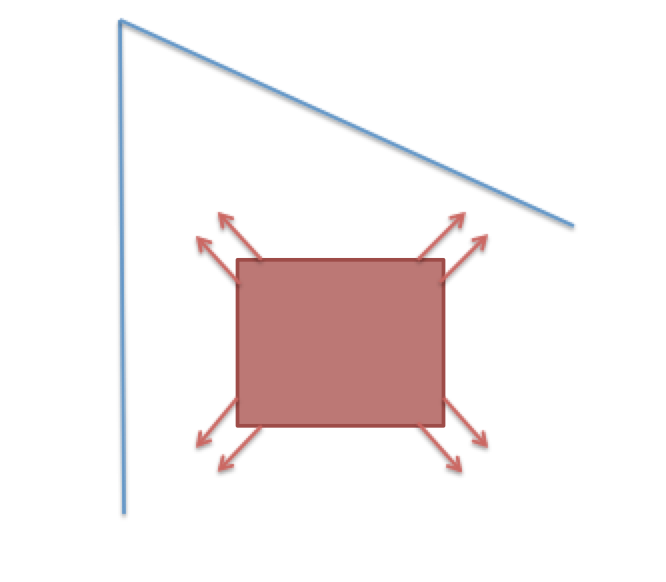
\includegraphics[width=.6\linewidth]{images/flatArea.png}
	\caption{Flat Area}
	\label{fig:flatArea}
\end{minipage}%
\begin{minipage}{.5\textwidth}
	\centering
	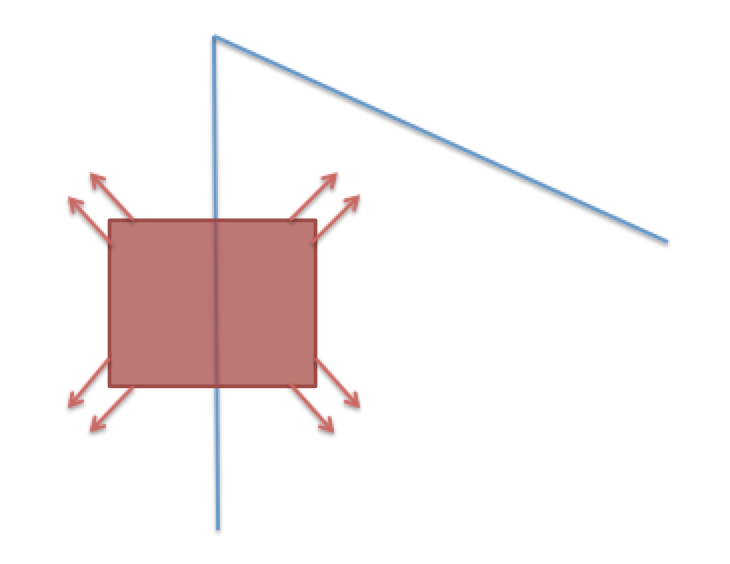
\includegraphics[width=.6\linewidth]{images/edgeArea.png}
	\caption{Edge Area}
	\label{fig:edgeArea}
\end{minipage}
\begin{minipage}{.5\textwidth}
	\centering
	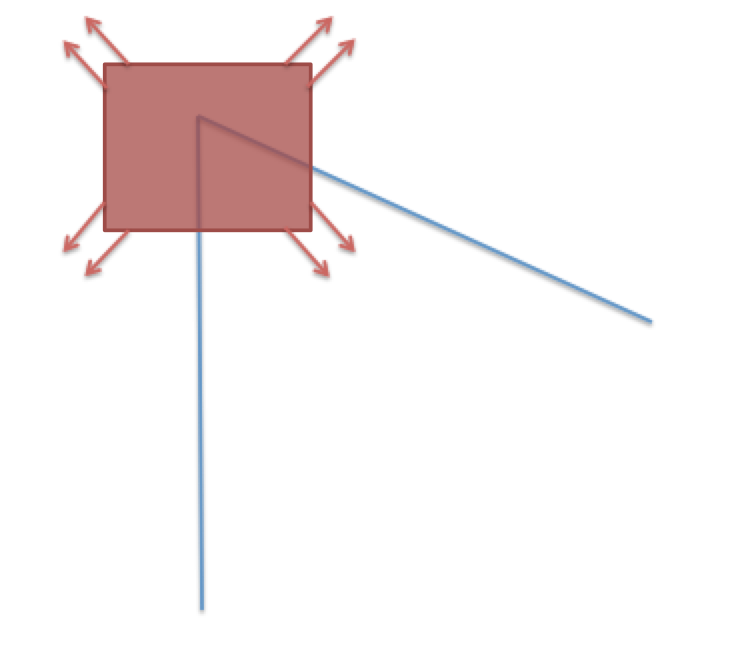
\includegraphics[width=.6\linewidth]{images/cornerArea.png}
	\caption{Corner Area}
	\label{fig:cornerArea}
\end{minipage}
\end{figure}


\section{Scale Invariant Feature Transform}
\subsection{Keypoint localization}
Although the $Harris\ corner\ detection$ algorithm presented in the previous section is immune to rotation transformations of an image, it does not perform well if the image is scaled, because a high intensity change in an area of size $(w, h)$ of an image might vary if the dimensions of the image change, but the size of the area remains the same.\\
Thus, D. Lowe, in 2004, presented a new algorithm for extracting keypoints and computing their descriptors, named $Scale\ Invariant\ Feature\ Transform$.\\
At first, a Gaussian distribution is applied on the analyzed image, which depending of the standard deviation, $\sigma$, blurs the image with a certain amount: $G(x, y) = \frac{1}{2 * \pi * \sigma^2} * e^{-\frac{x^2 + y^2}{2 * \sigma^2}}$.\\
Then, the Laplacian of the image is computed, in order to highlight the regions of rapid intensity changes: $L(x, y) = \frac{\delta^2 I}{\delta x^2} + \frac{\delta^2 I}{\delta y^2}$. Combined with the previous Gaussian filter, we obtain the so called Laplacian of Gaussian: $LoG(x, y) = -\frac{1}{\pi * \sigma^4} * \left(1 - \frac{x^2 + y^2}{2 * \sigma^2}\right) * e^{-\frac{x^2 + y^2}{2 * \sigma^2}}$.\\
Because the $LoG$ has a high computational cost, it is approximated with a Difference of Gaussians, which is a difference of two Gaussians with two different $\sigma$ deviations, representing two different scaled images. The local extrema of the computed $DoG$ are considered potential keypoints.
\subsection{Computing the Descriptors}
Once we have the keypoints, the corresponding descriptors are computed by taking a $16\times16$ neighborhood around the keypoint, and creating a $8$ bin histogram for each sub-block of $4\times4$ size of the initial neighbourhood. Thus, a keypoint descriptor will contain $128$ values.
